% generated by Plantuml 1.2025.2       
\definecolor{plantucolor0000}{RGB}{0,0,0}
\definecolor{plantucolor0001}{RGB}{255,255,255}
\definecolor{plantucolor0002}{RGB}{24,24,24}
\definecolor{plantucolor0003}{RGB}{226,226,240}
\definecolor{plantucolor0004}{RGB}{238,238,238}
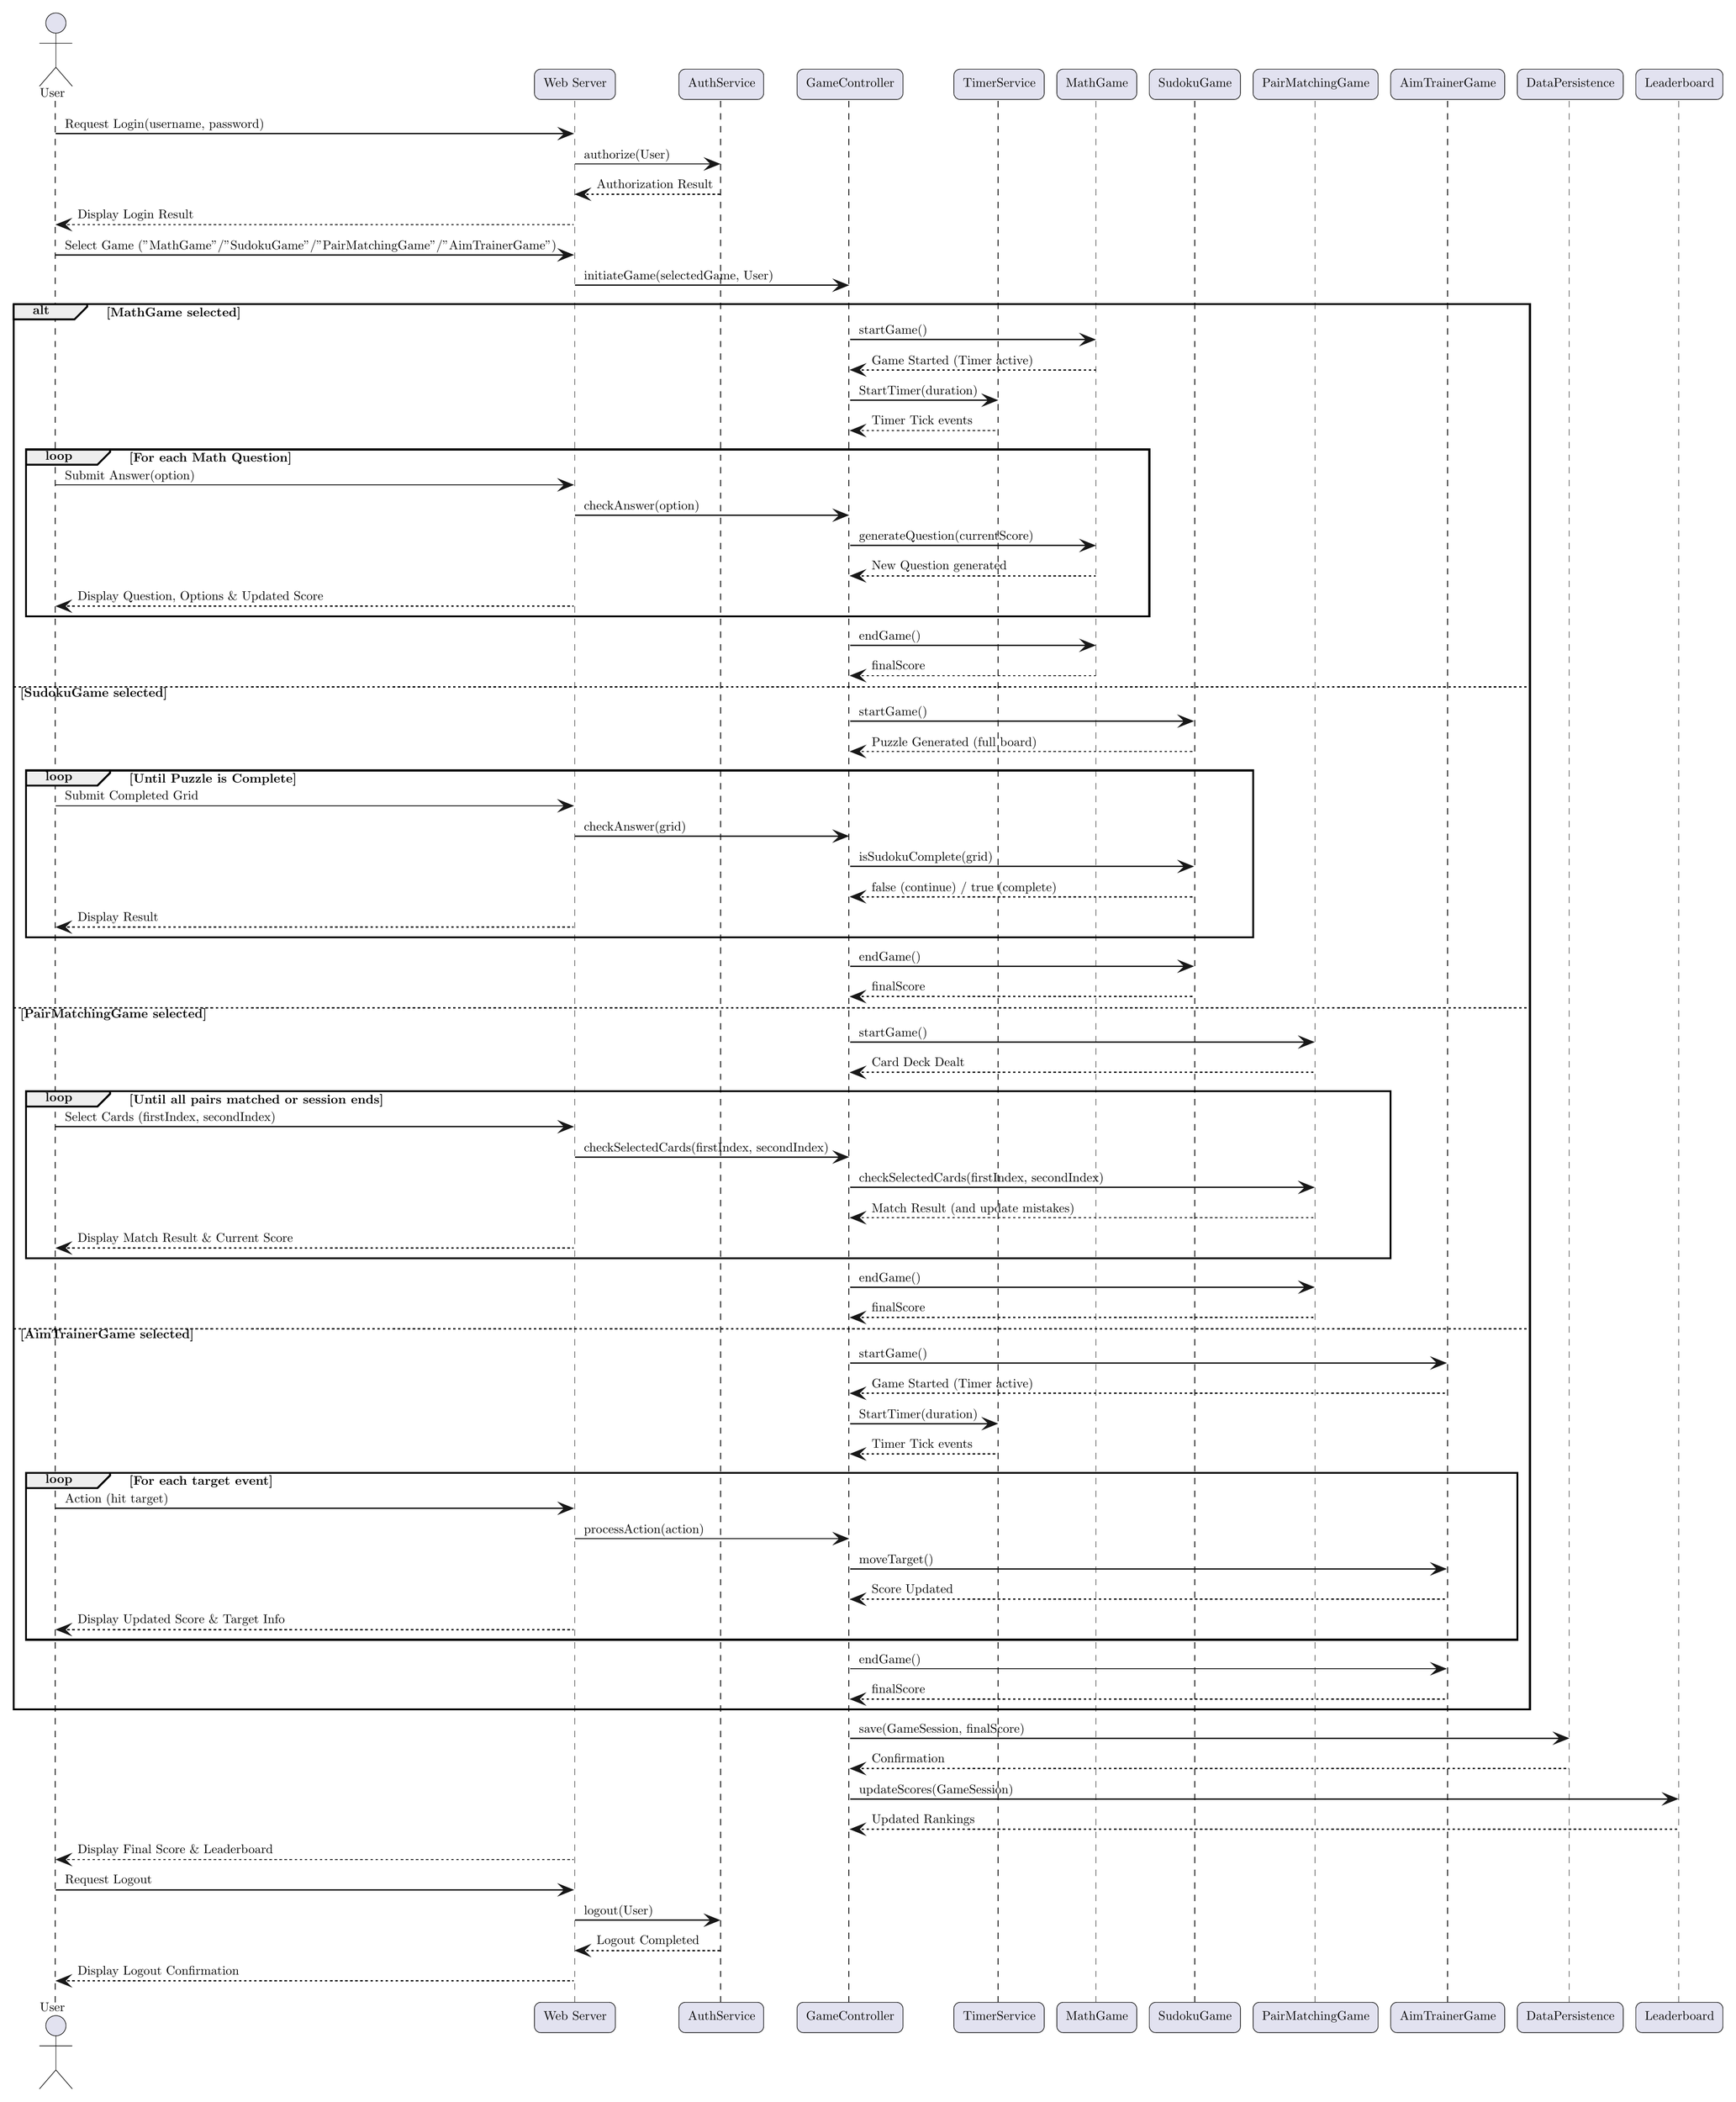
\begin{tikzpicture}[yscale=-1
,pstyle0/.style={color=black,line width=1.5pt}
,pstyle1/.style={color=plantucolor0001,line width=0.0pt}
,pstyle2/.style={color=plantucolor0002,line width=0.5pt,dash pattern=on 5.0pt off 5.0pt}
,pstyle3/.style={color=plantucolor0002,fill=plantucolor0003,line width=0.5pt}
,pstyle4/.style={color=plantucolor0002,line width=0.5pt}
,pstyle5/.style={color=plantucolor0002,fill=plantucolor0002,line width=1.0pt}
,pstyle6/.style={color=plantucolor0002,line width=1.0pt}
,pstyle7/.style={color=plantucolor0002,line width=1.0pt,dash pattern=on 2.0pt off 2.0pt}
,pstyle8/.style={color=black,fill=plantucolor0004,line width=1.5pt}
,pstyle9/.style={color=black,line width=1.0pt,dash pattern=on 2.0pt off 2.0pt}
]
\draw[pstyle0] (10pt,236pt) rectangle (1210.655pt,1348pt);
\draw[pstyle0] (20pt,351pt) rectangle (909.305pt,483pt);
\draw[pstyle0] (20pt,605pt) rectangle (991.445pt,737pt);
\draw[pstyle0] (20pt,859pt) rectangle (1100.415pt,991pt);
\draw[pstyle0] (20pt,1161pt) rectangle (1200.655pt,1293pt);
\draw[pstyle1] (39.5pt,75pt) rectangle (47.5pt,1581pt);
\draw[pstyle2] (43pt,75pt) -- (43pt,1581pt);
\draw[pstyle1] (450.46pt,75pt) rectangle (458.46pt,1581pt);
\draw[pstyle2] (454.43pt,75pt) -- (454.43pt,1581pt);
\draw[pstyle1] (566.36pt,75pt) rectangle (574.36pt,1581pt);
\draw[pstyle2] (569.815pt,75pt) -- (569.815pt,1581pt);
\draw[pstyle1] (668.29pt,75pt) rectangle (676.29pt,1581pt);
\draw[pstyle2] (671.365pt,75pt) -- (671.365pt,1581pt);
\draw[pstyle1] (786.29pt,75pt) rectangle (794.29pt,1581pt);
\draw[pstyle2] (789.515pt,75pt) -- (789.515pt,1581pt);
\draw[pstyle1] (863.685pt,75pt) rectangle (871.685pt,1581pt);
\draw[pstyle2] (867.065pt,75pt) -- (867.065pt,1581pt);
\draw[pstyle1] (941.375pt,75pt) rectangle (949.375pt,1581pt);
\draw[pstyle2] (945.305pt,75pt) -- (945.305pt,1581pt);
\draw[pstyle1] (1036.93pt,75pt) rectangle (1044.93pt,1581pt);
\draw[pstyle2] (1040.445pt,75pt) -- (1040.445pt,1581pt);
\draw[pstyle1] (1141.535pt,75pt) rectangle (1149.535pt,1581pt);
\draw[pstyle2] (1145.415pt,75pt) -- (1145.415pt,1581pt);
\draw[pstyle1] (1238.58pt,75pt) rectangle (1246.58pt,1581pt);
\draw[pstyle2] (1241.655pt,75pt) -- (1241.655pt,1581pt);
\draw[pstyle1] (1324.97pt,75pt) rectangle (1332.97pt,1581pt);
\draw[pstyle2] (1328.505pt,75pt) -- (1328.505pt,1581pt);
\node at (30.6pt,65pt)[below right,color=black,inner sep=0]{User};
\draw[pstyle3] (43.5pt,13.5pt) ellipse (8pt and 8pt);
\draw[pstyle4] (43.5pt,21.5pt) -- (43.5pt,48.5pt)(30.5pt,29.5pt) -- (56.5pt,29.5pt)(43.5pt,48.5pt) -- (30.5pt,63.5pt)(43.5pt,48.5pt) -- (56.5pt,63.5pt);
\node at (30.6pt,1580pt)[below right,color=black,inner sep=0]{User};
\draw[pstyle3] (43.5pt,1598.5pt) ellipse (8pt and 8pt);
\draw[pstyle4] (43.5pt,1606.5pt) -- (43.5pt,1633.5pt)(30.5pt,1614.5pt) -- (56.5pt,1614.5pt)(43.5pt,1633.5pt) -- (30.5pt,1648.5pt)(43.5pt,1633.5pt) -- (56.5pt,1648.5pt);
\draw[pstyle3] (422.43pt,55pt) arc (180:270:5pt) -- (427.43pt,50pt) -- (481.49pt,50pt) arc (270:360:5pt) -- (486.49pt,55pt) -- (486.49pt,69pt) arc (0:90:5pt) -- (481.49pt,74pt) -- (427.43pt,74pt) arc (90:180:5pt) -- (422.43pt,69pt) -- cycle;
\node at (429.43pt,57pt)[below right,color=black,inner sep=0]{Web Server};
\draw[pstyle3] (422.43pt,1585pt) arc (180:270:5pt) -- (427.43pt,1580pt) -- (481.49pt,1580pt) arc (270:360:5pt) -- (486.49pt,1585pt) -- (486.49pt,1599pt) arc (0:90:5pt) -- (481.49pt,1604pt) -- (427.43pt,1604pt) arc (90:180:5pt) -- (422.43pt,1599pt) -- cycle;
\node at (429.43pt,1587pt)[below right,color=black,inner sep=0]{Web Server};
\draw[pstyle3] (536.815pt,55pt) arc (180:270:5pt) -- (541.815pt,50pt) -- (598.905pt,50pt) arc (270:360:5pt) -- (603.905pt,55pt) -- (603.905pt,69pt) arc (0:90:5pt) -- (598.905pt,74pt) -- (541.815pt,74pt) arc (90:180:5pt) -- (536.815pt,69pt) -- cycle;
\node at (543.815pt,57pt)[below right,color=black,inner sep=0]{AuthService};
\draw[pstyle3] (536.815pt,1585pt) arc (180:270:5pt) -- (541.815pt,1580pt) -- (598.905pt,1580pt) arc (270:360:5pt) -- (603.905pt,1585pt) -- (603.905pt,1599pt) arc (0:90:5pt) -- (598.905pt,1604pt) -- (541.815pt,1604pt) arc (90:180:5pt) -- (536.815pt,1599pt) -- cycle;
\node at (543.815pt,1587pt)[below right,color=black,inner sep=0]{AuthService};
\draw[pstyle3] (630.365pt,55pt) arc (180:270:5pt) -- (635.365pt,50pt) -- (709.215pt,50pt) arc (270:360:5pt) -- (714.215pt,55pt) -- (714.215pt,69pt) arc (0:90:5pt) -- (709.215pt,74pt) -- (635.365pt,74pt) arc (90:180:5pt) -- (630.365pt,69pt) -- cycle;
\node at (637.365pt,57pt)[below right,color=black,inner sep=0]{GameController};
\draw[pstyle3] (630.365pt,1585pt) arc (180:270:5pt) -- (635.365pt,1580pt) -- (709.215pt,1580pt) arc (270:360:5pt) -- (714.215pt,1585pt) -- (714.215pt,1599pt) arc (0:90:5pt) -- (709.215pt,1604pt) -- (635.365pt,1604pt) arc (90:180:5pt) -- (630.365pt,1599pt) -- cycle;
\node at (637.365pt,1587pt)[below right,color=black,inner sep=0]{GameController};
\draw[pstyle3] (754.515pt,55pt) arc (180:270:5pt) -- (759.515pt,50pt) -- (821.065pt,50pt) arc (270:360:5pt) -- (826.065pt,55pt) -- (826.065pt,69pt) arc (0:90:5pt) -- (821.065pt,74pt) -- (759.515pt,74pt) arc (90:180:5pt) -- (754.515pt,69pt) -- cycle;
\node at (761.515pt,57pt)[below right,color=black,inner sep=0]{TimerService};
\draw[pstyle3] (754.515pt,1585pt) arc (180:270:5pt) -- (759.515pt,1580pt) -- (821.065pt,1580pt) arc (270:360:5pt) -- (826.065pt,1585pt) -- (826.065pt,1599pt) arc (0:90:5pt) -- (821.065pt,1604pt) -- (759.515pt,1604pt) arc (90:180:5pt) -- (754.515pt,1599pt) -- cycle;
\node at (761.515pt,1587pt)[below right,color=black,inner sep=0]{TimerService};
\draw[pstyle3] (836.065pt,55pt) arc (180:270:5pt) -- (841.065pt,50pt) -- (894.305pt,50pt) arc (270:360:5pt) -- (899.305pt,55pt) -- (899.305pt,69pt) arc (0:90:5pt) -- (894.305pt,74pt) -- (841.065pt,74pt) arc (90:180:5pt) -- (836.065pt,69pt) -- cycle;
\node at (843.065pt,57pt)[below right,color=black,inner sep=0]{MathGame};
\draw[pstyle3] (836.065pt,1585pt) arc (180:270:5pt) -- (841.065pt,1580pt) -- (894.305pt,1580pt) arc (270:360:5pt) -- (899.305pt,1585pt) -- (899.305pt,1599pt) arc (0:90:5pt) -- (894.305pt,1604pt) -- (841.065pt,1604pt) arc (90:180:5pt) -- (836.065pt,1599pt) -- cycle;
\node at (843.065pt,1587pt)[below right,color=black,inner sep=0]{MathGame};
\draw[pstyle3] (909.305pt,55pt) arc (180:270:5pt) -- (914.305pt,50pt) -- (976.445pt,50pt) arc (270:360:5pt) -- (981.445pt,55pt) -- (981.445pt,69pt) arc (0:90:5pt) -- (976.445pt,74pt) -- (914.305pt,74pt) arc (90:180:5pt) -- (909.305pt,69pt) -- cycle;
\node at (916.305pt,57pt)[below right,color=black,inner sep=0]{SudokuGame};
\draw[pstyle3] (909.305pt,1585pt) arc (180:270:5pt) -- (914.305pt,1580pt) -- (976.445pt,1580pt) arc (270:360:5pt) -- (981.445pt,1585pt) -- (981.445pt,1599pt) arc (0:90:5pt) -- (976.445pt,1604pt) -- (914.305pt,1604pt) arc (90:180:5pt) -- (909.305pt,1599pt) -- cycle;
\node at (916.305pt,1587pt)[below right,color=black,inner sep=0]{SudokuGame};
\draw[pstyle3] (991.445pt,55pt) arc (180:270:5pt) -- (996.445pt,50pt) -- (1085.415pt,50pt) arc (270:360:5pt) -- (1090.415pt,55pt) -- (1090.415pt,69pt) arc (0:90:5pt) -- (1085.415pt,74pt) -- (996.445pt,74pt) arc (90:180:5pt) -- (991.445pt,69pt) -- cycle;
\node at (998.445pt,57pt)[below right,color=black,inner sep=0]{PairMatchingGame};
\draw[pstyle3] (991.445pt,1585pt) arc (180:270:5pt) -- (996.445pt,1580pt) -- (1085.415pt,1580pt) arc (270:360:5pt) -- (1090.415pt,1585pt) -- (1090.415pt,1599pt) arc (0:90:5pt) -- (1085.415pt,1604pt) -- (996.445pt,1604pt) arc (90:180:5pt) -- (991.445pt,1599pt) -- cycle;
\node at (998.445pt,1587pt)[below right,color=black,inner sep=0]{PairMatchingGame};
\draw[pstyle3] (1100.415pt,55pt) arc (180:270:5pt) -- (1105.415pt,50pt) -- (1185.655pt,50pt) arc (270:360:5pt) -- (1190.655pt,55pt) -- (1190.655pt,69pt) arc (0:90:5pt) -- (1185.655pt,74pt) -- (1105.415pt,74pt) arc (90:180:5pt) -- (1100.415pt,69pt) -- cycle;
\node at (1107.415pt,57pt)[below right,color=black,inner sep=0]{AimTrainerGame};
\draw[pstyle3] (1100.415pt,1585pt) arc (180:270:5pt) -- (1105.415pt,1580pt) -- (1185.655pt,1580pt) arc (270:360:5pt) -- (1190.655pt,1585pt) -- (1190.655pt,1599pt) arc (0:90:5pt) -- (1185.655pt,1604pt) -- (1105.415pt,1604pt) arc (90:180:5pt) -- (1100.415pt,1599pt) -- cycle;
\node at (1107.415pt,1587pt)[below right,color=black,inner sep=0]{AimTrainerGame};
\draw[pstyle3] (1200.655pt,55pt) arc (180:270:5pt) -- (1205.655pt,50pt) -- (1279.505pt,50pt) arc (270:360:5pt) -- (1284.505pt,55pt) -- (1284.505pt,69pt) arc (0:90:5pt) -- (1279.505pt,74pt) -- (1205.655pt,74pt) arc (90:180:5pt) -- (1200.655pt,69pt) -- cycle;
\node at (1207.655pt,57pt)[below right,color=black,inner sep=0]{DataPersistence};
\draw[pstyle3] (1200.655pt,1585pt) arc (180:270:5pt) -- (1205.655pt,1580pt) -- (1279.505pt,1580pt) arc (270:360:5pt) -- (1284.505pt,1585pt) -- (1284.505pt,1599pt) arc (0:90:5pt) -- (1279.505pt,1604pt) -- (1205.655pt,1604pt) arc (90:180:5pt) -- (1200.655pt,1599pt) -- cycle;
\node at (1207.655pt,1587pt)[below right,color=black,inner sep=0]{DataPersistence};
\draw[pstyle3] (1294.505pt,55pt) arc (180:270:5pt) -- (1299.505pt,50pt) -- (1358.435pt,50pt) arc (270:360:5pt) -- (1363.435pt,55pt) -- (1363.435pt,69pt) arc (0:90:5pt) -- (1358.435pt,74pt) -- (1299.505pt,74pt) arc (90:180:5pt) -- (1294.505pt,69pt) -- cycle;
\node at (1301.505pt,57pt)[below right,color=black,inner sep=0]{Leaderboard};
\draw[pstyle3] (1294.505pt,1585pt) arc (180:270:5pt) -- (1299.505pt,1580pt) -- (1358.435pt,1580pt) arc (270:360:5pt) -- (1363.435pt,1585pt) -- (1363.435pt,1599pt) arc (0:90:5pt) -- (1358.435pt,1604pt) -- (1299.505pt,1604pt) arc (90:180:5pt) -- (1294.505pt,1599pt) -- cycle;
\node at (1301.505pt,1587pt)[below right,color=black,inner sep=0]{Leaderboard};
\draw[pstyle5] (442.46pt,97pt) -- (452.46pt,101pt) -- (442.46pt,105pt) -- (446.46pt,101pt) -- cycle;
\draw[pstyle6] (43.5pt,101pt) -- (448.46pt,101pt);
\node at (50.5pt,89pt)[below right,color=black,inner sep=0]{Request Login(username, password)};
\draw[pstyle5] (558.36pt,121pt) -- (568.36pt,125pt) -- (558.36pt,129pt) -- (562.36pt,125pt) -- cycle;
\draw[pstyle6] (454.46pt,125pt) -- (564.36pt,125pt);
\node at (461.46pt,113pt)[below right,color=black,inner sep=0]{authorize(User)};
\draw[pstyle5] (465.46pt,145pt) -- (455.46pt,149pt) -- (465.46pt,153pt) -- (461.46pt,149pt) -- cycle;
\draw[pstyle7] (459.46pt,149pt) -- (569.36pt,149pt);
\node at (471.46pt,137pt)[below right,color=black,inner sep=0]{Authorization Result};
\draw[pstyle5] (54.5pt,169pt) -- (44.5pt,173pt) -- (54.5pt,177pt) -- (50.5pt,173pt) -- cycle;
\draw[pstyle7] (48.5pt,173pt) -- (453.46pt,173pt);
\node at (60.5pt,161pt)[below right,color=black,inner sep=0]{Display Login Result};
\draw[pstyle5] (442.46pt,193pt) -- (452.46pt,197pt) -- (442.46pt,201pt) -- (446.46pt,197pt) -- cycle;
\draw[pstyle6] (43.5pt,197pt) -- (448.46pt,197pt);
\node at (50.5pt,185pt)[below right,color=black,inner sep=0]{Select Game ("MathGame"/"SudokuGame"/"PairMatchingGame"/"AimTrainerGame")};
\draw[pstyle5] (660.29pt,217pt) -- (670.29pt,221pt) -- (660.29pt,225pt) -- (664.29pt,221pt) -- cycle;
\draw[pstyle6] (454.46pt,221pt) -- (666.29pt,221pt);
\node at (461.46pt,209pt)[below right,color=black,inner sep=0]{initiateGame(selectedGame, User)};
\draw[pstyle8] (10pt,236pt) -- (68.25pt,236pt) -- (68.25pt,238pt) -- (58.25pt,248pt) -- (10pt,248pt) -- (10pt,236pt);
\draw[pstyle0] (10pt,236pt) rectangle (1210.655pt,1348pt);
\node at (25pt,237pt)[below right,color=black,inner sep=0]{\textbf{alt}};
\node at (83.25pt,238pt)[below right,color=black,inner sep=0]{\textbf{[MathGame selected]}};
\draw[pstyle5] (855.685pt,260pt) -- (865.685pt,264pt) -- (855.685pt,268pt) -- (859.685pt,264pt) -- cycle;
\draw[pstyle6] (672.29pt,264pt) -- (861.685pt,264pt);
\node at (679.29pt,252pt)[below right,color=black,inner sep=0]{startGame()};
\draw[pstyle5] (683.29pt,284pt) -- (673.29pt,288pt) -- (683.29pt,292pt) -- (679.29pt,288pt) -- cycle;
\draw[pstyle7] (677.29pt,288pt) -- (866.685pt,288pt);
\node at (689.29pt,276pt)[below right,color=black,inner sep=0]{Game Started (Timer active)};
\draw[pstyle5] (778.29pt,308pt) -- (788.29pt,312pt) -- (778.29pt,316pt) -- (782.29pt,312pt) -- cycle;
\draw[pstyle6] (672.29pt,312pt) -- (784.29pt,312pt);
\node at (679.29pt,300pt)[below right,color=black,inner sep=0]{StartTimer(duration)};
\draw[pstyle5] (683.29pt,332pt) -- (673.29pt,336pt) -- (683.29pt,340pt) -- (679.29pt,336pt) -- cycle;
\draw[pstyle7] (677.29pt,336pt) -- (789.29pt,336pt);
\node at (689.29pt,324pt)[below right,color=black,inner sep=0]{Timer Tick events};
\draw[pstyle8] (20pt,351pt) -- (86.4pt,351pt) -- (86.4pt,353pt) -- (76.4pt,363pt) -- (20pt,363pt) -- (20pt,351pt);
\draw[pstyle0] (20pt,351pt) rectangle (909.305pt,483pt);
\node at (35pt,352pt)[below right,color=black,inner sep=0]{\textbf{loop}};
\node at (101.4pt,353pt)[below right,color=black,inner sep=0]{\textbf{[For each Math Question]}};
\draw[pstyle5] (442.46pt,375pt) -- (452.46pt,379pt) -- (442.46pt,383pt) -- (446.46pt,379pt) -- cycle;
\draw[pstyle6] (43.5pt,379pt) -- (448.46pt,379pt);
\node at (50.5pt,367pt)[below right,color=black,inner sep=0]{Submit Answer(option)};
\draw[pstyle5] (660.29pt,399pt) -- (670.29pt,403pt) -- (660.29pt,407pt) -- (664.29pt,403pt) -- cycle;
\draw[pstyle6] (454.46pt,403pt) -- (666.29pt,403pt);
\node at (461.46pt,391pt)[below right,color=black,inner sep=0]{checkAnswer(option)};
\draw[pstyle5] (855.685pt,423pt) -- (865.685pt,427pt) -- (855.685pt,431pt) -- (859.685pt,427pt) -- cycle;
\draw[pstyle6] (672.29pt,427pt) -- (861.685pt,427pt);
\node at (679.29pt,415pt)[below right,color=black,inner sep=0]{generateQuestion(currentScore)};
\draw[pstyle5] (683.29pt,447pt) -- (673.29pt,451pt) -- (683.29pt,455pt) -- (679.29pt,451pt) -- cycle;
\draw[pstyle7] (677.29pt,451pt) -- (866.685pt,451pt);
\node at (689.29pt,439pt)[below right,color=black,inner sep=0]{New Question generated};
\draw[pstyle5] (54.5pt,471pt) -- (44.5pt,475pt) -- (54.5pt,479pt) -- (50.5pt,475pt) -- cycle;
\draw[pstyle7] (48.5pt,475pt) -- (453.46pt,475pt);
\node at (60.5pt,463pt)[below right,color=black,inner sep=0]{Display Question, Options \& Updated Score};
\draw[pstyle5] (855.685pt,502pt) -- (865.685pt,506pt) -- (855.685pt,510pt) -- (859.685pt,506pt) -- cycle;
\draw[pstyle6] (672.29pt,506pt) -- (861.685pt,506pt);
\node at (679.29pt,494pt)[below right,color=black,inner sep=0]{endGame()};
\draw[pstyle5] (683.29pt,526pt) -- (673.29pt,530pt) -- (683.29pt,534pt) -- (679.29pt,530pt) -- cycle;
\draw[pstyle7] (677.29pt,530pt) -- (866.685pt,530pt);
\node at (689.29pt,518pt)[below right,color=black,inner sep=0]{finalScore};
\draw[pstyle9] (10pt,539pt) -- (1210.655pt,539pt);
\node at (15pt,539pt)[below right,color=black,inner sep=0]{\textbf{[SudokuGame selected]}};
\draw[pstyle5] (933.375pt,562pt) -- (943.375pt,566pt) -- (933.375pt,570pt) -- (937.375pt,566pt) -- cycle;
\draw[pstyle6] (672.29pt,566pt) -- (939.375pt,566pt);
\node at (679.29pt,554pt)[below right,color=black,inner sep=0]{startGame()};
\draw[pstyle5] (683.29pt,586pt) -- (673.29pt,590pt) -- (683.29pt,594pt) -- (679.29pt,590pt) -- cycle;
\draw[pstyle7] (677.29pt,590pt) -- (944.375pt,590pt);
\node at (689.29pt,578pt)[below right,color=black,inner sep=0]{Puzzle Generated (full board)};
\draw[pstyle8] (20pt,605pt) -- (86.4pt,605pt) -- (86.4pt,607pt) -- (76.4pt,617pt) -- (20pt,617pt) -- (20pt,605pt);
\draw[pstyle0] (20pt,605pt) rectangle (991.445pt,737pt);
\node at (35pt,606pt)[below right,color=black,inner sep=0]{\textbf{loop}};
\node at (101.4pt,607pt)[below right,color=black,inner sep=0]{\textbf{[Until Puzzle is Complete]}};
\draw[pstyle5] (442.46pt,629pt) -- (452.46pt,633pt) -- (442.46pt,637pt) -- (446.46pt,633pt) -- cycle;
\draw[pstyle6] (43.5pt,633pt) -- (448.46pt,633pt);
\node at (50.5pt,621pt)[below right,color=black,inner sep=0]{Submit Completed Grid};
\draw[pstyle5] (660.29pt,653pt) -- (670.29pt,657pt) -- (660.29pt,661pt) -- (664.29pt,657pt) -- cycle;
\draw[pstyle6] (454.46pt,657pt) -- (666.29pt,657pt);
\node at (461.46pt,645pt)[below right,color=black,inner sep=0]{checkAnswer(grid)};
\draw[pstyle5] (933.375pt,677pt) -- (943.375pt,681pt) -- (933.375pt,685pt) -- (937.375pt,681pt) -- cycle;
\draw[pstyle6] (672.29pt,681pt) -- (939.375pt,681pt);
\node at (679.29pt,669pt)[below right,color=black,inner sep=0]{isSudokuComplete(grid)};
\draw[pstyle5] (683.29pt,701pt) -- (673.29pt,705pt) -- (683.29pt,709pt) -- (679.29pt,705pt) -- cycle;
\draw[pstyle7] (677.29pt,705pt) -- (944.375pt,705pt);
\node at (689.29pt,693pt)[below right,color=black,inner sep=0]{false (continue) / true (complete)};
\draw[pstyle5] (54.5pt,725pt) -- (44.5pt,729pt) -- (54.5pt,733pt) -- (50.5pt,729pt) -- cycle;
\draw[pstyle7] (48.5pt,729pt) -- (453.46pt,729pt);
\node at (60.5pt,717pt)[below right,color=black,inner sep=0]{Display Result};
\draw[pstyle5] (933.375pt,756pt) -- (943.375pt,760pt) -- (933.375pt,764pt) -- (937.375pt,760pt) -- cycle;
\draw[pstyle6] (672.29pt,760pt) -- (939.375pt,760pt);
\node at (679.29pt,748pt)[below right,color=black,inner sep=0]{endGame()};
\draw[pstyle5] (683.29pt,780pt) -- (673.29pt,784pt) -- (683.29pt,788pt) -- (679.29pt,784pt) -- cycle;
\draw[pstyle7] (677.29pt,784pt) -- (944.375pt,784pt);
\node at (689.29pt,772pt)[below right,color=black,inner sep=0]{finalScore};
\draw[pstyle9] (10pt,793pt) -- (1210.655pt,793pt);
\node at (15pt,793pt)[below right,color=black,inner sep=0]{\textbf{[PairMatchingGame selected]}};
\draw[pstyle5] (1028.93pt,816pt) -- (1038.93pt,820pt) -- (1028.93pt,824pt) -- (1032.93pt,820pt) -- cycle;
\draw[pstyle6] (672.29pt,820pt) -- (1034.93pt,820pt);
\node at (679.29pt,808pt)[below right,color=black,inner sep=0]{startGame()};
\draw[pstyle5] (683.29pt,840pt) -- (673.29pt,844pt) -- (683.29pt,848pt) -- (679.29pt,844pt) -- cycle;
\draw[pstyle7] (677.29pt,844pt) -- (1039.93pt,844pt);
\node at (689.29pt,832pt)[below right,color=black,inner sep=0]{Card Deck Dealt};
\draw[pstyle8] (20pt,859pt) -- (86.4pt,859pt) -- (86.4pt,861pt) -- (76.4pt,871pt) -- (20pt,871pt) -- (20pt,859pt);
\draw[pstyle0] (20pt,859pt) rectangle (1100.415pt,991pt);
\node at (35pt,860pt)[below right,color=black,inner sep=0]{\textbf{loop}};
\node at (101.4pt,861pt)[below right,color=black,inner sep=0]{\textbf{[Until all pairs matched or session ends]}};
\draw[pstyle5] (442.46pt,883pt) -- (452.46pt,887pt) -- (442.46pt,891pt) -- (446.46pt,887pt) -- cycle;
\draw[pstyle6] (43.5pt,887pt) -- (448.46pt,887pt);
\node at (50.5pt,875pt)[below right,color=black,inner sep=0]{Select Cards (firstIndex, secondIndex)};
\draw[pstyle5] (660.29pt,907pt) -- (670.29pt,911pt) -- (660.29pt,915pt) -- (664.29pt,911pt) -- cycle;
\draw[pstyle6] (454.46pt,911pt) -- (666.29pt,911pt);
\node at (461.46pt,899pt)[below right,color=black,inner sep=0]{checkSelectedCards(firstIndex, secondIndex)};
\draw[pstyle5] (1028.93pt,931pt) -- (1038.93pt,935pt) -- (1028.93pt,939pt) -- (1032.93pt,935pt) -- cycle;
\draw[pstyle6] (672.29pt,935pt) -- (1034.93pt,935pt);
\node at (679.29pt,923pt)[below right,color=black,inner sep=0]{checkSelectedCards(firstIndex, secondIndex)};
\draw[pstyle5] (683.29pt,955pt) -- (673.29pt,959pt) -- (683.29pt,963pt) -- (679.29pt,959pt) -- cycle;
\draw[pstyle7] (677.29pt,959pt) -- (1039.93pt,959pt);
\node at (689.29pt,947pt)[below right,color=black,inner sep=0]{Match Result (and update mistakes)};
\draw[pstyle5] (54.5pt,979pt) -- (44.5pt,983pt) -- (54.5pt,987pt) -- (50.5pt,983pt) -- cycle;
\draw[pstyle7] (48.5pt,983pt) -- (453.46pt,983pt);
\node at (60.5pt,971pt)[below right,color=black,inner sep=0]{Display Match Result \& Current Score};
\draw[pstyle5] (1028.93pt,1010pt) -- (1038.93pt,1014pt) -- (1028.93pt,1018pt) -- (1032.93pt,1014pt) -- cycle;
\draw[pstyle6] (672.29pt,1014pt) -- (1034.93pt,1014pt);
\node at (679.29pt,1002pt)[below right,color=black,inner sep=0]{endGame()};
\draw[pstyle5] (683.29pt,1034pt) -- (673.29pt,1038pt) -- (683.29pt,1042pt) -- (679.29pt,1038pt) -- cycle;
\draw[pstyle7] (677.29pt,1038pt) -- (1039.93pt,1038pt);
\node at (689.29pt,1026pt)[below right,color=black,inner sep=0]{finalScore};
\draw[pstyle9] (10pt,1047pt) -- (1210.655pt,1047pt);
\node at (15pt,1047pt)[below right,color=black,inner sep=0]{\textbf{[AimTrainerGame selected]}};
\draw[pstyle5] (1133.535pt,1070pt) -- (1143.535pt,1074pt) -- (1133.535pt,1078pt) -- (1137.535pt,1074pt) -- cycle;
\draw[pstyle6] (672.29pt,1074pt) -- (1139.535pt,1074pt);
\node at (679.29pt,1062pt)[below right,color=black,inner sep=0]{startGame()};
\draw[pstyle5] (683.29pt,1094pt) -- (673.29pt,1098pt) -- (683.29pt,1102pt) -- (679.29pt,1098pt) -- cycle;
\draw[pstyle7] (677.29pt,1098pt) -- (1144.535pt,1098pt);
\node at (689.29pt,1086pt)[below right,color=black,inner sep=0]{Game Started (Timer active)};
\draw[pstyle5] (778.29pt,1118pt) -- (788.29pt,1122pt) -- (778.29pt,1126pt) -- (782.29pt,1122pt) -- cycle;
\draw[pstyle6] (672.29pt,1122pt) -- (784.29pt,1122pt);
\node at (679.29pt,1110pt)[below right,color=black,inner sep=0]{StartTimer(duration)};
\draw[pstyle5] (683.29pt,1142pt) -- (673.29pt,1146pt) -- (683.29pt,1150pt) -- (679.29pt,1146pt) -- cycle;
\draw[pstyle7] (677.29pt,1146pt) -- (789.29pt,1146pt);
\node at (689.29pt,1134pt)[below right,color=black,inner sep=0]{Timer Tick events};
\draw[pstyle8] (20pt,1161pt) -- (86.4pt,1161pt) -- (86.4pt,1163pt) -- (76.4pt,1173pt) -- (20pt,1173pt) -- (20pt,1161pt);
\draw[pstyle0] (20pt,1161pt) rectangle (1200.655pt,1293pt);
\node at (35pt,1162pt)[below right,color=black,inner sep=0]{\textbf{loop}};
\node at (101.4pt,1163pt)[below right,color=black,inner sep=0]{\textbf{[For each target event]}};
\draw[pstyle5] (442.46pt,1185pt) -- (452.46pt,1189pt) -- (442.46pt,1193pt) -- (446.46pt,1189pt) -- cycle;
\draw[pstyle6] (43.5pt,1189pt) -- (448.46pt,1189pt);
\node at (50.5pt,1177pt)[below right,color=black,inner sep=0]{Action (hit target)};
\draw[pstyle5] (660.29pt,1209pt) -- (670.29pt,1213pt) -- (660.29pt,1217pt) -- (664.29pt,1213pt) -- cycle;
\draw[pstyle6] (454.46pt,1213pt) -- (666.29pt,1213pt);
\node at (461.46pt,1201pt)[below right,color=black,inner sep=0]{processAction(action)};
\draw[pstyle5] (1133.535pt,1233pt) -- (1143.535pt,1237pt) -- (1133.535pt,1241pt) -- (1137.535pt,1237pt) -- cycle;
\draw[pstyle6] (672.29pt,1237pt) -- (1139.535pt,1237pt);
\node at (679.29pt,1225pt)[below right,color=black,inner sep=0]{moveTarget()};
\draw[pstyle5] (683.29pt,1257pt) -- (673.29pt,1261pt) -- (683.29pt,1265pt) -- (679.29pt,1261pt) -- cycle;
\draw[pstyle7] (677.29pt,1261pt) -- (1144.535pt,1261pt);
\node at (689.29pt,1249pt)[below right,color=black,inner sep=0]{Score Updated};
\draw[pstyle5] (54.5pt,1281pt) -- (44.5pt,1285pt) -- (54.5pt,1289pt) -- (50.5pt,1285pt) -- cycle;
\draw[pstyle7] (48.5pt,1285pt) -- (453.46pt,1285pt);
\node at (60.5pt,1273pt)[below right,color=black,inner sep=0]{Display Updated Score \& Target Info};
\draw[pstyle5] (1133.535pt,1312pt) -- (1143.535pt,1316pt) -- (1133.535pt,1320pt) -- (1137.535pt,1316pt) -- cycle;
\draw[pstyle6] (672.29pt,1316pt) -- (1139.535pt,1316pt);
\node at (679.29pt,1304pt)[below right,color=black,inner sep=0]{endGame()};
\draw[pstyle5] (683.29pt,1336pt) -- (673.29pt,1340pt) -- (683.29pt,1344pt) -- (679.29pt,1340pt) -- cycle;
\draw[pstyle7] (677.29pt,1340pt) -- (1144.535pt,1340pt);
\node at (689.29pt,1328pt)[below right,color=black,inner sep=0]{finalScore};
\draw[pstyle5] (1230.58pt,1367pt) -- (1240.58pt,1371pt) -- (1230.58pt,1375pt) -- (1234.58pt,1371pt) -- cycle;
\draw[pstyle6] (672.29pt,1371pt) -- (1236.58pt,1371pt);
\node at (679.29pt,1359pt)[below right,color=black,inner sep=0]{save(GameSession, finalScore)};
\draw[pstyle5] (683.29pt,1391pt) -- (673.29pt,1395pt) -- (683.29pt,1399pt) -- (679.29pt,1395pt) -- cycle;
\draw[pstyle7] (677.29pt,1395pt) -- (1241.58pt,1395pt);
\node at (689.29pt,1383pt)[below right,color=black,inner sep=0]{Confirmation};
\draw[pstyle5] (1316.97pt,1415pt) -- (1326.97pt,1419pt) -- (1316.97pt,1423pt) -- (1320.97pt,1419pt) -- cycle;
\draw[pstyle6] (672.29pt,1419pt) -- (1322.97pt,1419pt);
\node at (679.29pt,1407pt)[below right,color=black,inner sep=0]{updateScores(GameSession)};
\draw[pstyle5] (683.29pt,1439pt) -- (673.29pt,1443pt) -- (683.29pt,1447pt) -- (679.29pt,1443pt) -- cycle;
\draw[pstyle7] (677.29pt,1443pt) -- (1327.97pt,1443pt);
\node at (689.29pt,1431pt)[below right,color=black,inner sep=0]{Updated Rankings};
\draw[pstyle5] (54.5pt,1463pt) -- (44.5pt,1467pt) -- (54.5pt,1471pt) -- (50.5pt,1467pt) -- cycle;
\draw[pstyle7] (48.5pt,1467pt) -- (453.46pt,1467pt);
\node at (60.5pt,1455pt)[below right,color=black,inner sep=0]{Display Final Score \& Leaderboard};
\draw[pstyle5] (442.46pt,1487pt) -- (452.46pt,1491pt) -- (442.46pt,1495pt) -- (446.46pt,1491pt) -- cycle;
\draw[pstyle6] (43.5pt,1491pt) -- (448.46pt,1491pt);
\node at (50.5pt,1479pt)[below right,color=black,inner sep=0]{Request Logout};
\draw[pstyle5] (558.36pt,1511pt) -- (568.36pt,1515pt) -- (558.36pt,1519pt) -- (562.36pt,1515pt) -- cycle;
\draw[pstyle6] (454.46pt,1515pt) -- (564.36pt,1515pt);
\node at (461.46pt,1503pt)[below right,color=black,inner sep=0]{logout(User)};
\draw[pstyle5] (465.46pt,1535pt) -- (455.46pt,1539pt) -- (465.46pt,1543pt) -- (461.46pt,1539pt) -- cycle;
\draw[pstyle7] (459.46pt,1539pt) -- (569.36pt,1539pt);
\node at (471.46pt,1527pt)[below right,color=black,inner sep=0]{Logout Completed};
\draw[pstyle5] (54.5pt,1559pt) -- (44.5pt,1563pt) -- (54.5pt,1567pt) -- (50.5pt,1563pt) -- cycle;
\draw[pstyle7] (48.5pt,1563pt) -- (453.46pt,1563pt);
\node at (60.5pt,1551pt)[below right,color=black,inner sep=0]{Display Logout Confirmation};
\end{tikzpicture}
